In this section we compare the Standard Model Higgs exclusion limits
for different channels.

\begin{figure}[!hbtp]

\centering
\subfigure[SF 0-Jet Cut]{
\centering
\label{subfig:sf_0j_cut}
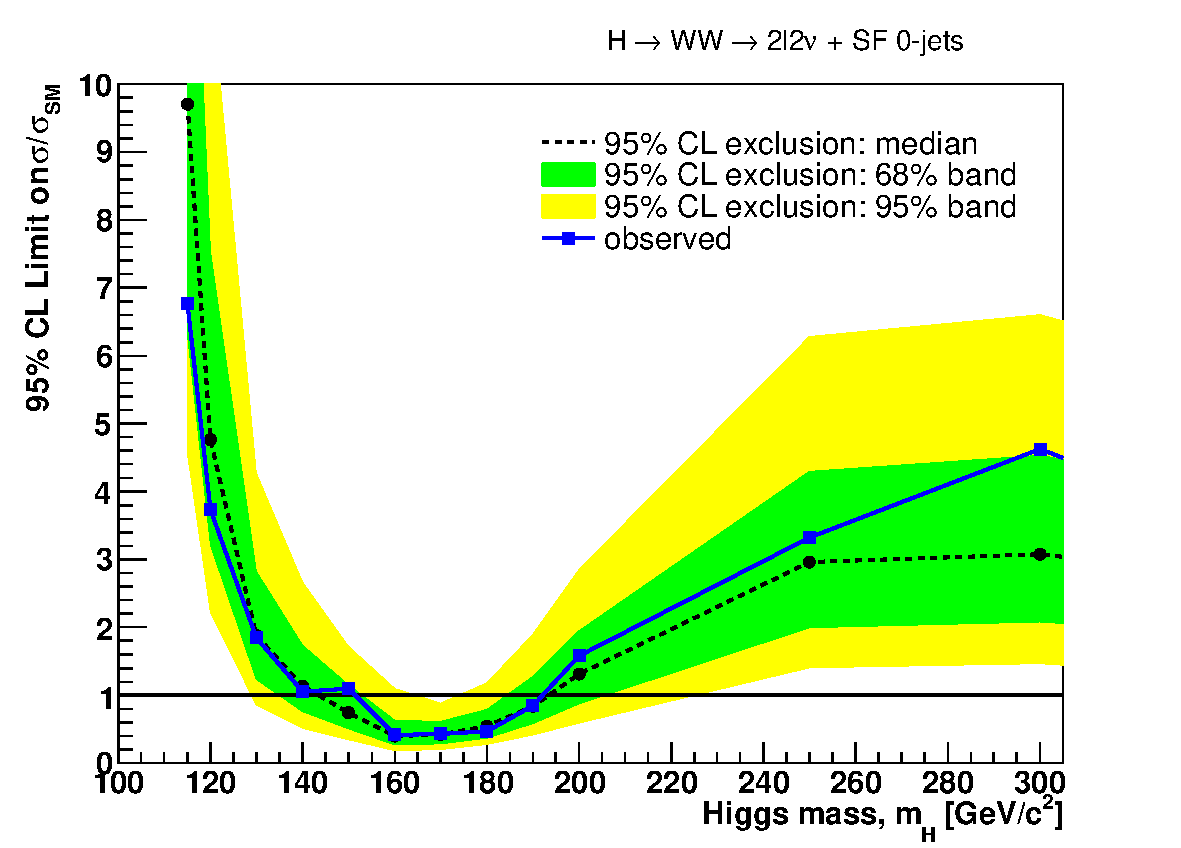
\includegraphics[width=.45\textwidth]{figures/limits_sf_0j_cut.pdf}}
\subfigure[OF 0-Jet Cut]{
\centering
\label{subfig:of_0j_cut}
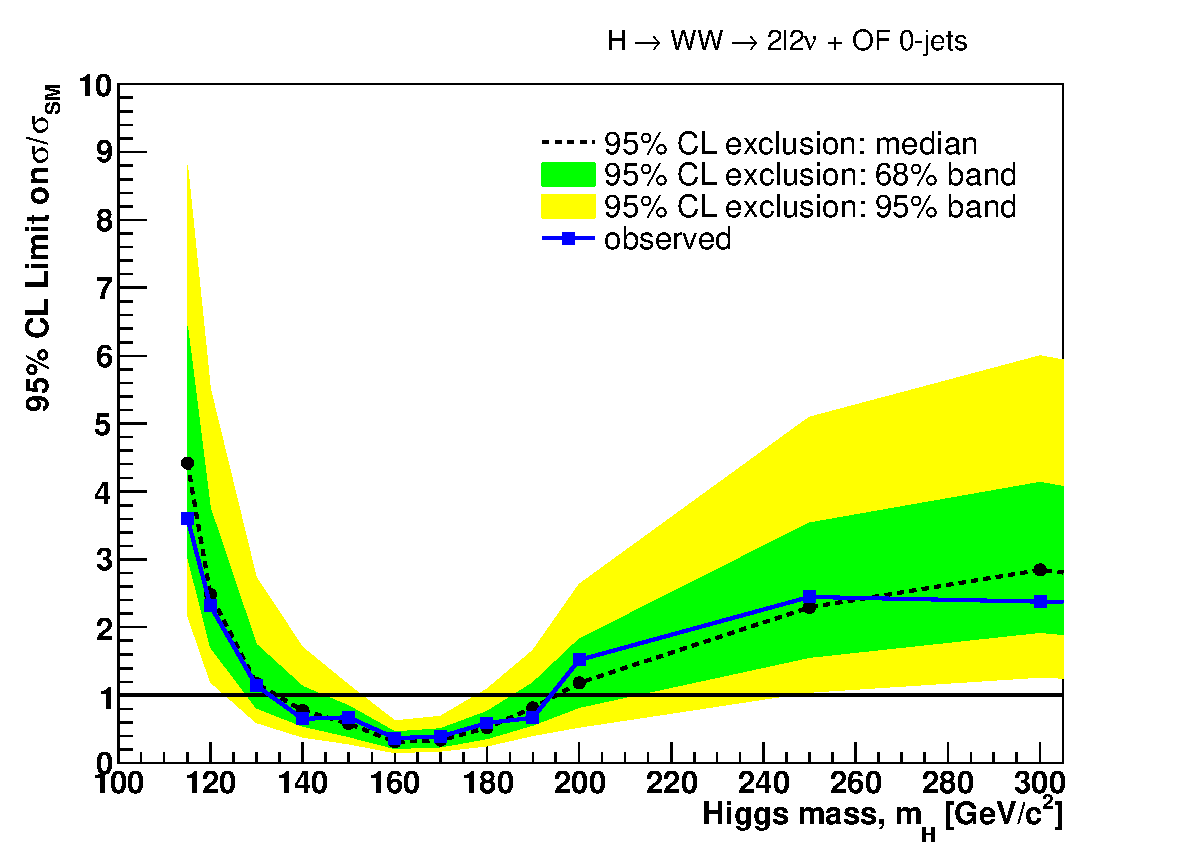
\includegraphics[width=.45\textwidth]{figures/limits_of_0j_cut.pdf}}
\subfigure[SF 1-Jet Cut]{
\centering
\label{subfig:sf_1j_cut}
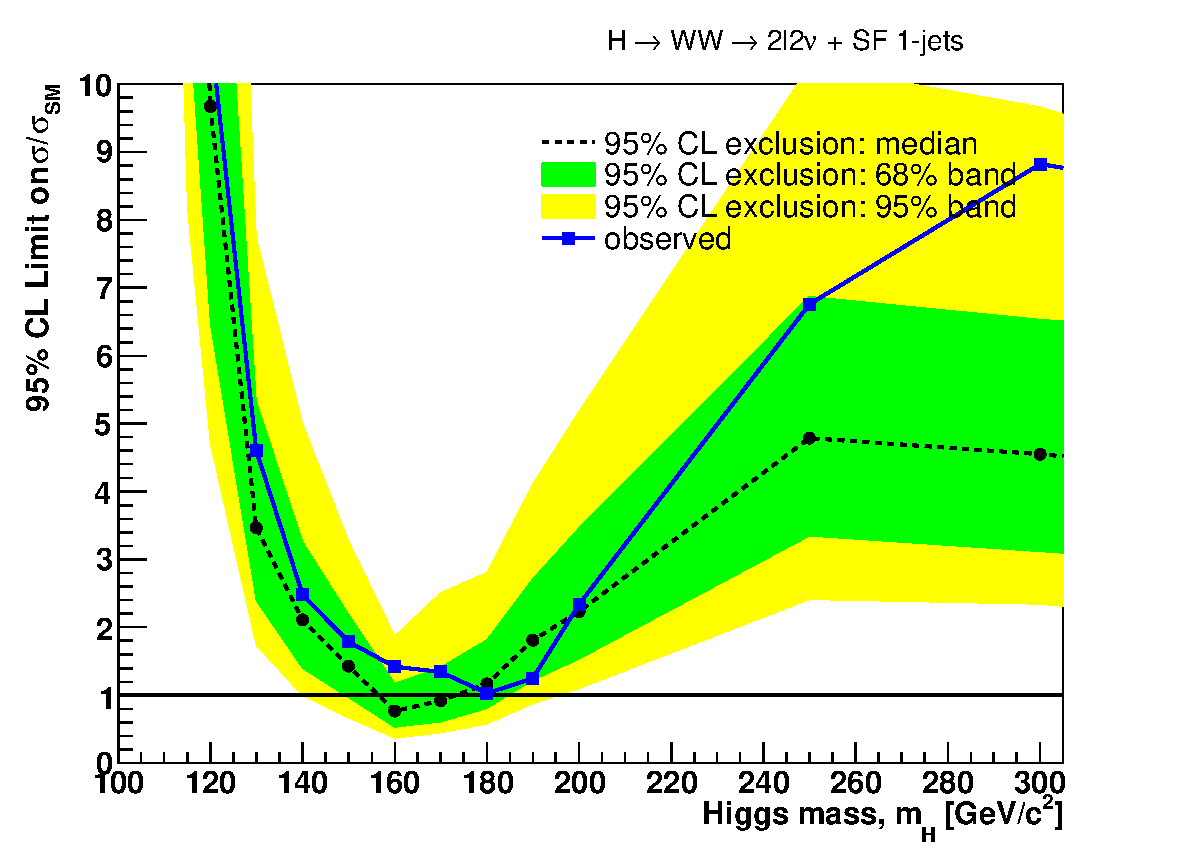
\includegraphics[width=.45\textwidth]{figures/limits_sf_1j_cut.pdf}}
\subfigure[OF 1-Jet Cut]{
\centering
\label{subfig:of_1j_cut}
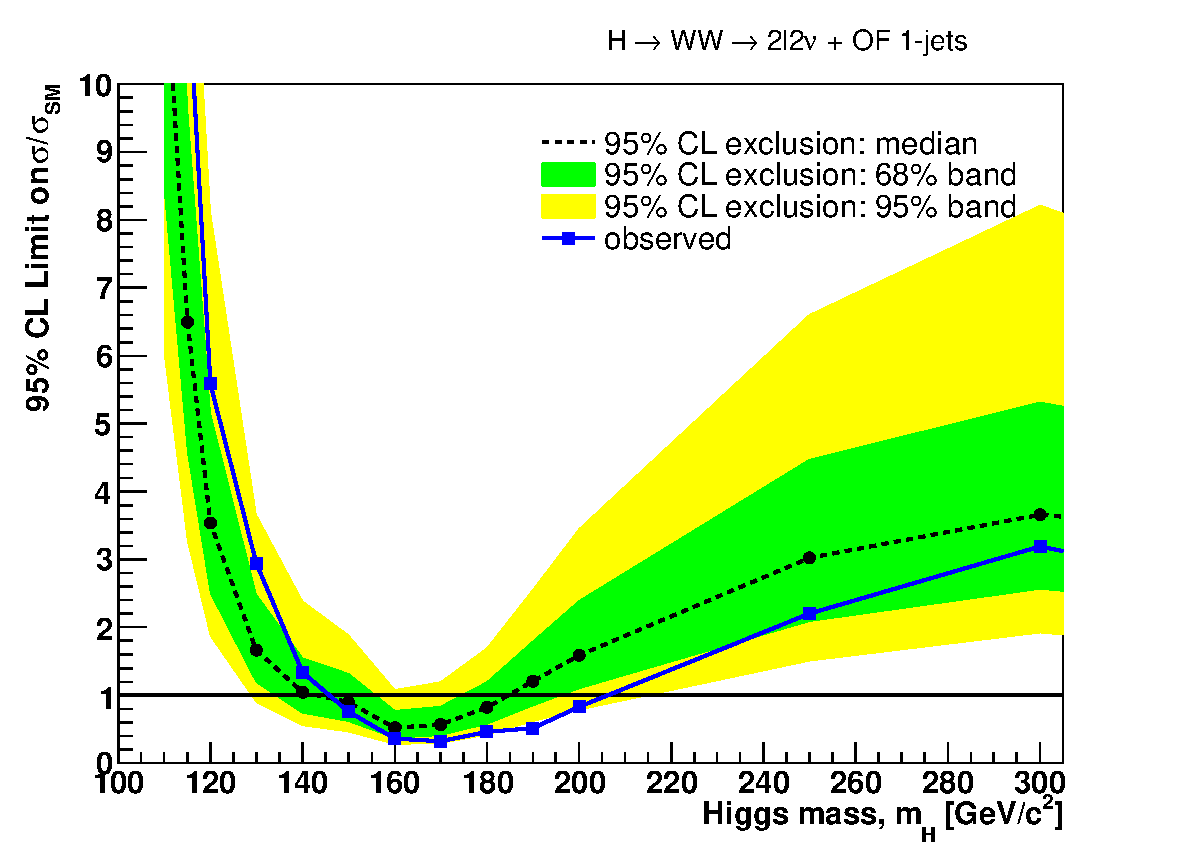
\includegraphics[width=.45\textwidth]{figures/limits_of_1j_cut.pdf}}
\subfigure[2-Jet Cut]{
\centering
\label{subfig:vbf_2j_cut}
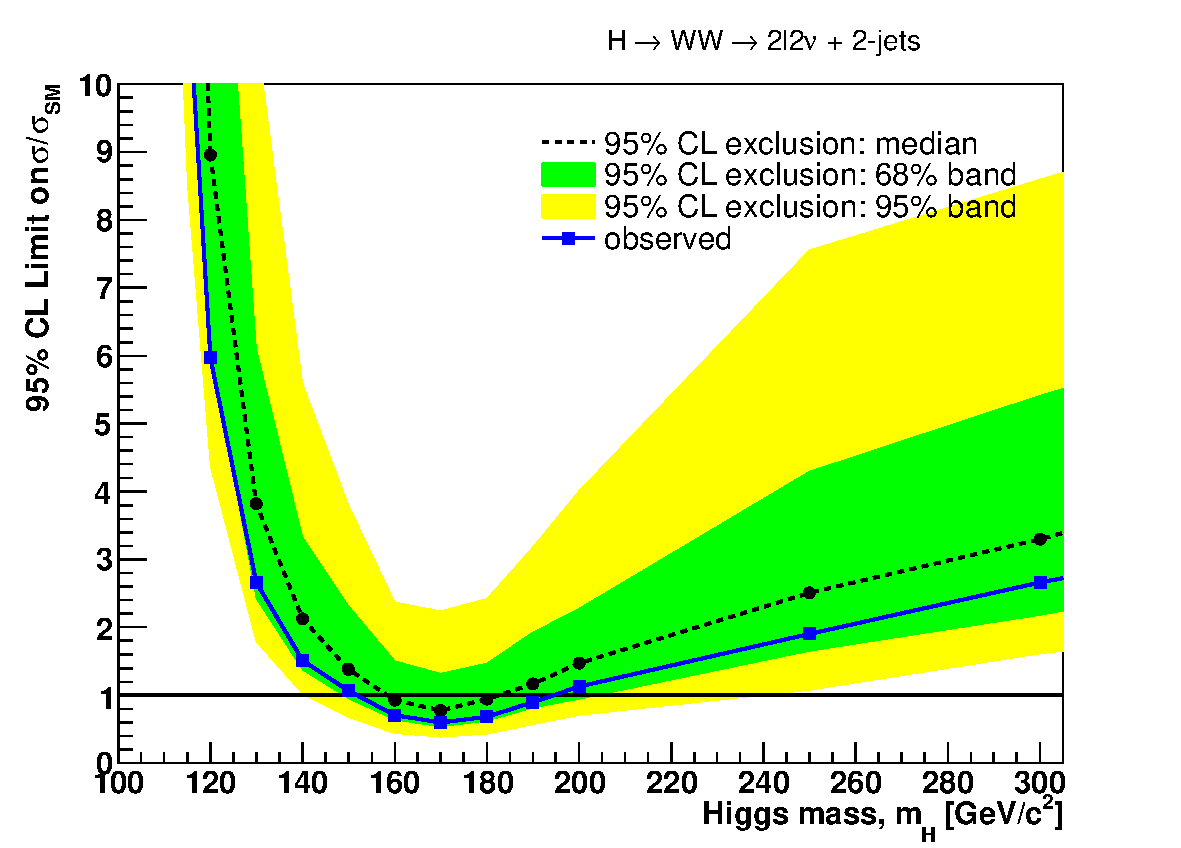
\includegraphics[width=.45\textwidth]{figures/limits_2j_cut.pdf}}
\caption{Expected and observed upper limits on the SM Higgs
  cross-section for the {\bf cut-based} analysis.}
\label{fig:ul_cutbased_subchannels}
\end{figure}

\begin{figure}[!hbtp]

\centering
\subfigure[SF 0-Jet Shape]{
\centering
\label{subfig:sf_0j_shape}
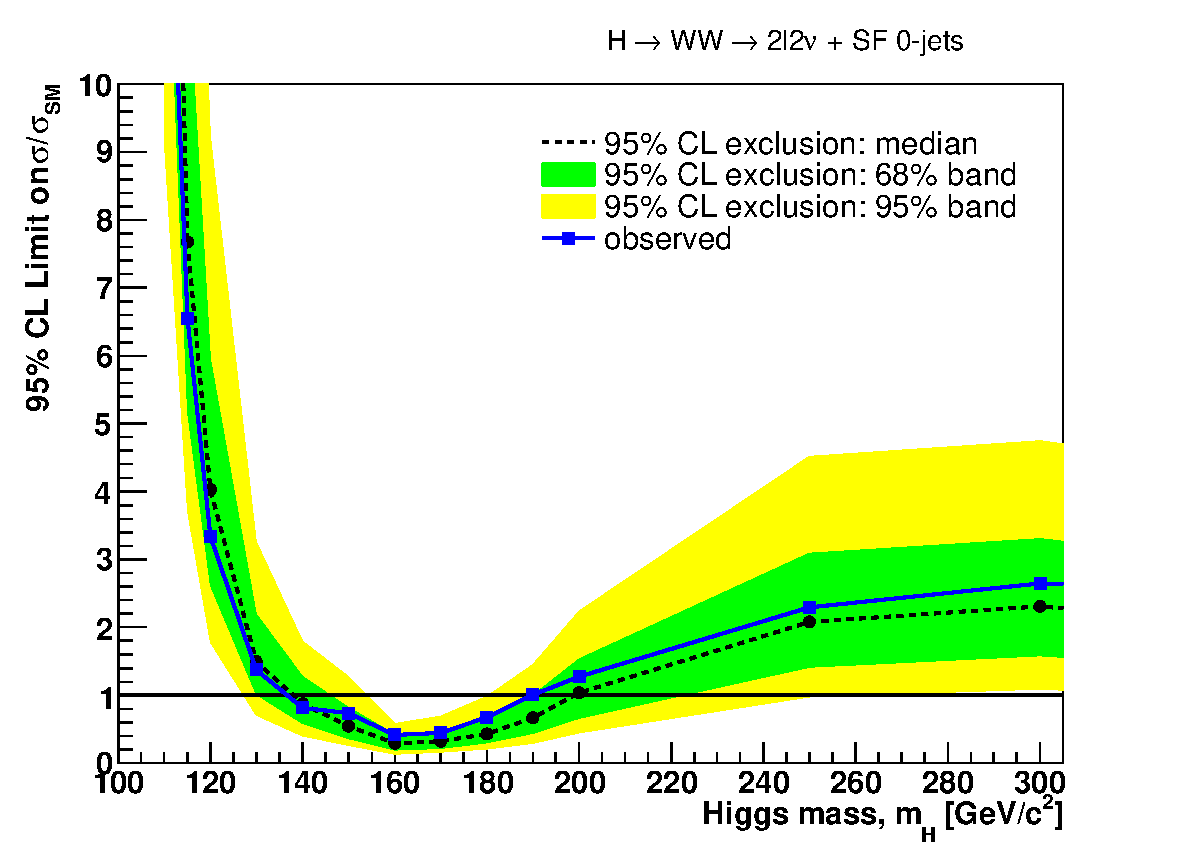
\includegraphics[width=.45\textwidth]{figures/limits_sf_0j_shape.pdf}}
\subfigure[OF 0-Jet Shape]{
\centering
\label{subfig:of_0j_shape}
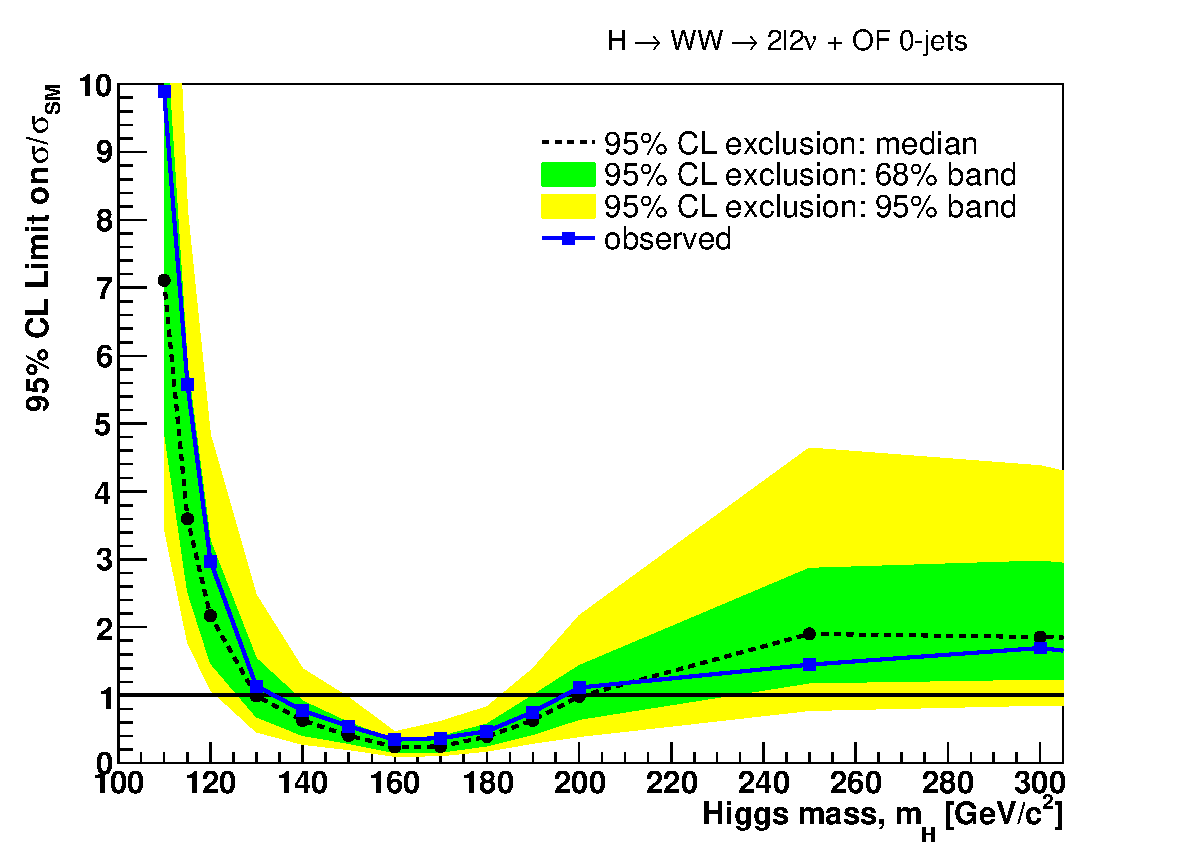
\includegraphics[width=.45\textwidth]{figures/limits_of_0j_shape.pdf}}
\subfigure[SF 1-Jet Shape]{
\centering
\label{subfig:sf_1j_shape}
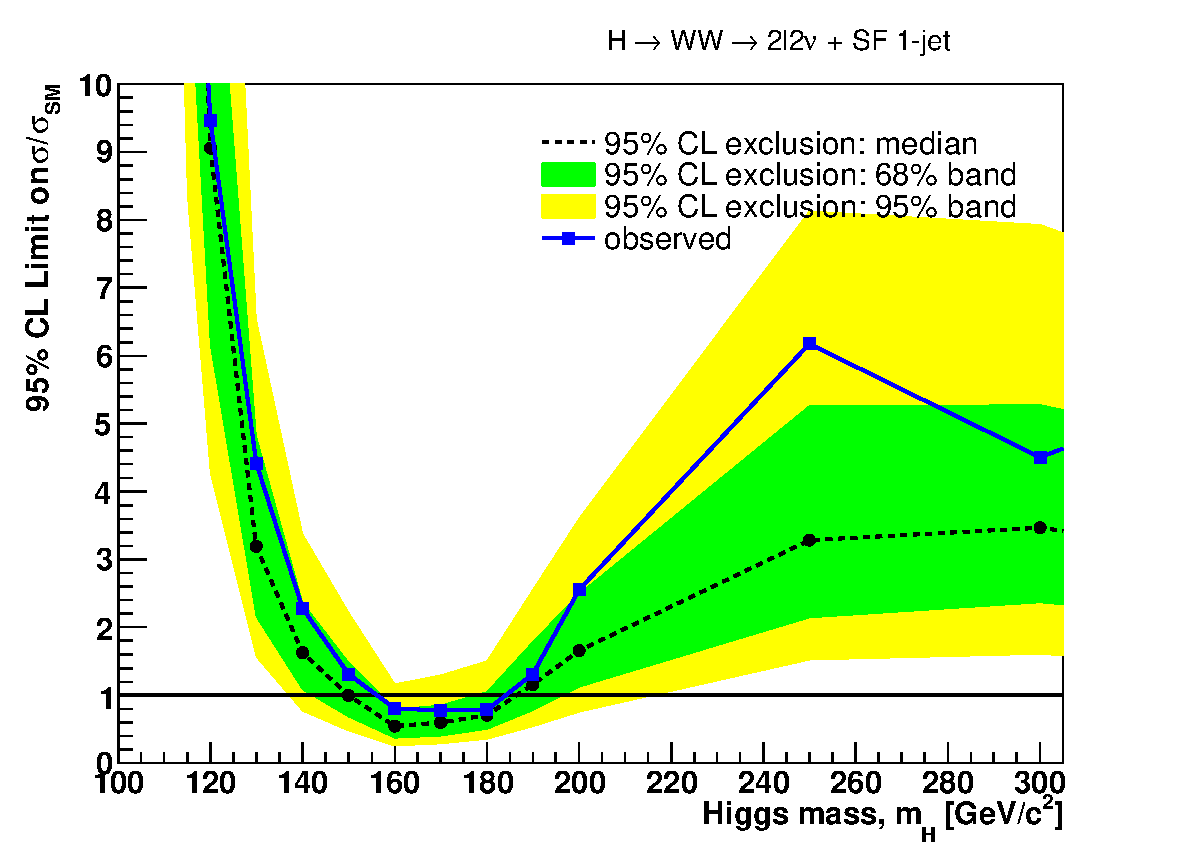
\includegraphics[width=.45\textwidth]{figures/limits_sf_1j_shape.pdf}}
\subfigure[OF 1-Jet Shape]{
\centering
\label{subfig:of_1j_shape}
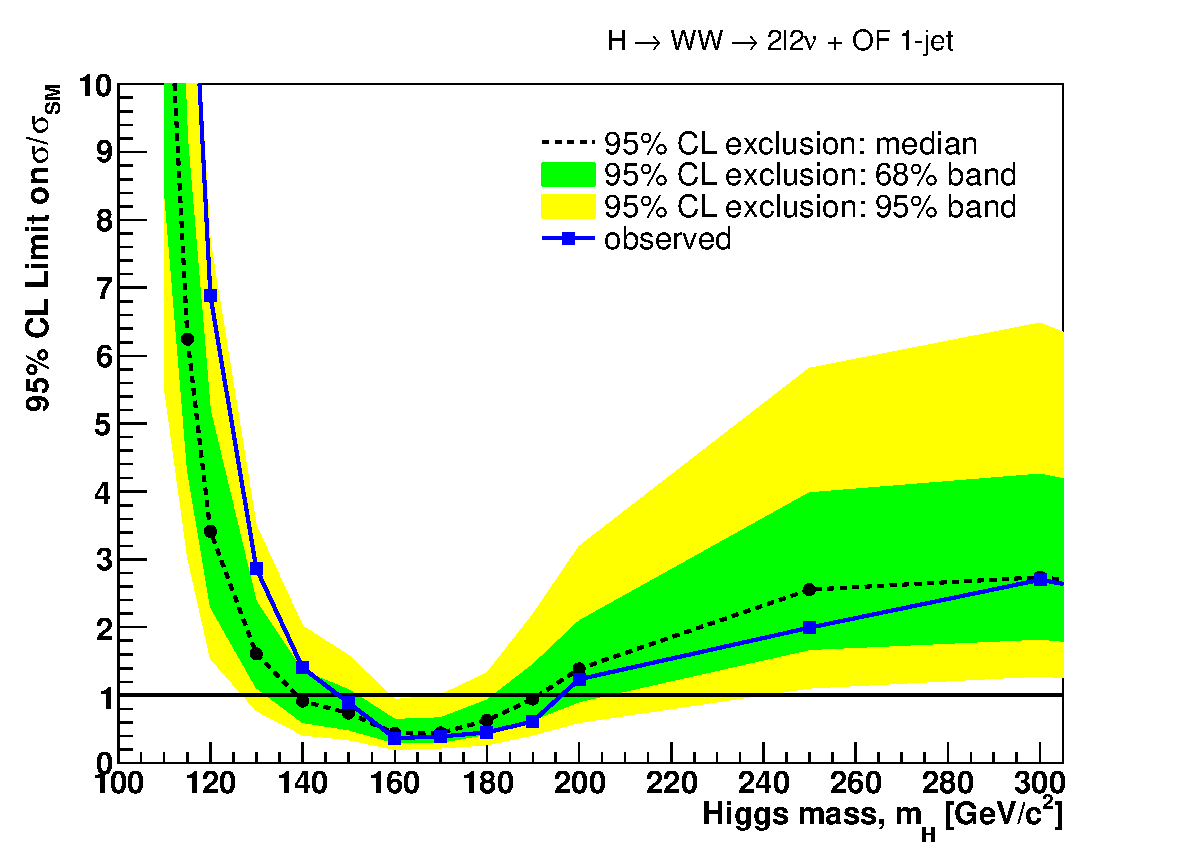
\includegraphics[width=.45\textwidth]{figures/limits_of_1j_shape.pdf}}
\caption{Expected and observed upper limits on the SM Higgs
  cross-section for the {\bf shape-based} analysis.}
\label{fig:ul_shapebased_subchannels}
\end{figure}


%%%%%%%%%%%%%%%%%%%%%%%%%%%%%%
\begin{table}[!hbp]
\begin{center}
\begin{tabular}{c c c c c}
\hline
\vspace{-3mm} && \\
 Higgs Mass   & Observed & Median expected & Expected range for 68\% & Expected range for 95\%   \\
\vspace{-3mm} && \\
\hline
110 & 16.1 & 23.1 & [15.0, 36.8] & [10.8, 60.2] \\
115 & 6.8 & 9.7 & [6.3, 15.4] & [4.6, 25.3] \\
120 & 3.7 & 4.8 & [3.2, 7.5] & [2.2, 11.5] \\
130 & 1.9 & 1.9 & [1.2, 2.8] & [0.9, 4.3] \\
140 & 1.0 & 1.1 & [0.8, 1.7] & [0.5, 2.7] \\
150 & 1.1 & 0.7 & [0.5, 1.2] & [0.3, 1.7] \\
160 & 0.4 & 0.4 & [0.3, 0.6] & [0.2, 1.1] \\
170 & 0.4 & 0.4 & [0.3, 0.6] & [0.2, 0.9] \\
180 & 0.5 & 0.5 & [0.4, 0.8] & [0.3, 1.2] \\
190 & 0.8 & 0.8 & [0.6, 1.3] & [0.4, 1.9] \\
200 & 1.6 & 1.3 & [0.9, 1.9] & [0.6, 2.9] \\
250 & 3.3 & 3.0 & [2.0, 4.3] & [1.4, 6.3] \\
300 & 4.6 & 3.1 & [2.1, 4.5] & [1.5, 6.6] \\
350 & 3.3 & 2.7 & [1.9, 3.9] & [1.2, 5.7] \\
400 & 3.2 & 2.9 & [2.1, 4.3] & [1.4, 6.5] \\
450 & 4.2 & 4.1 & [2.8, 6.2] & [2.1, 8.9] \\
500 & 7.4 & 5.9 & [4.2, 8.6] & [3.1, 12.6] \\
550 & 15.4 & 9.0 & [6.3, 13.8] & [4.7, 19.8] \\
600 & 18.6 & 14.1 & [9.7, 20.4] & [7.3, 30.3] \\
\hline
\end{tabular}
\caption{Expected and observed upper limits for {\bf cut-based 0-jet
    same-flavor} analysis with \intlumi\ of data}
\label{tab:sf0_cut}
\end{center}
\end{table}
%%%%%%%%%%%%%%%%%%%%%%%%%%%%%%

%%%%%%%%%%%%%%%%%%%%%%%%%%%%%%
\begin{table}[!hbp]
\begin{center}
\begin{tabular}{c c c c c}
\hline
\vspace{-3mm} && \\
 Higgs Mass   & Observed & Median expected & Expected range for 68\% & Expected range for 95\%   \\
\vspace{-3mm} && \\
\hline
110 & 7.4 & 9.1 & [6.3, 13.2] & [4.5, 18.1] \\
115 & 3.6 & 4.4 & [3.0, 6.4] & [2.2, 8.8] \\
120 & 2.3 & 2.5 & [1.7, 3.8] & [1.2, 5.5] \\
130 & 1.1 & 1.2 & [0.8, 1.7] & [0.6, 2.7] \\
140 & 0.7 & 0.8 & [0.5, 1.1] & [0.4, 1.7] \\
150 & 0.7 & 0.6 & [0.4, 0.8] & [0.3, 1.2] \\
160 & 0.4 & 0.3 & [0.2, 0.5] & [0.2, 0.6] \\
170 & 0.4 & 0.3 & [0.2, 0.5] & [0.2, 0.7] \\
180 & 0.6 & 0.5 & [0.4, 0.8] & [0.3, 1.1] \\
190 & 0.7 & 0.8 & [0.6, 1.2] & [0.4, 1.7] \\
200 & 1.5 & 1.2 & [0.8, 1.8] & [0.5, 2.6] \\
250 & 2.4 & 2.3 & [1.6, 3.5] & [1.0, 5.1] \\
300 & 2.4 & 2.8 & [1.9, 4.1] & [1.3, 6.0] \\
350 & 2.3 & 2.5 & [1.6, 3.5] & [1.2, 5.4] \\
400 & 2.8 & 2.7 & [1.8, 4.1] & [1.3, 5.9] \\
450 & 3.7 & 3.5 & [2.4, 5.4] & [1.7, 8.1] \\
500 & 4.1 & 5.3 & [3.6, 7.4] & [2.6, 10.7] \\
550 & 6.7 & 7.8 & [5.4, 12.2] & [3.8, 17.8] \\
600 & 12.6 & 11.7 & [8.1, 18.6] & [5.7, 27.1] \\
\hline
\end{tabular}
\caption{Expected and observed upper limits for {\bf cut-based 0-jet
    opposite-flavor} analysis with \intlumi\ of data}
\label{tab:of0_cut}
\end{center}
\end{table}
%%%%%%%%%%%%%%%%%%%%%%%%%%%%%%

%%%%%%%%%%%%%%%%%%%%%%%%%%%%%%
\begin{table}[!hbp]
\begin{center}
\begin{tabular}{c c c c c}
\hline
\vspace{-3mm} && \\
 Higgs Mass   & Observed & Median expected & Expected range for 68\% & Expected range for 95\%   \\
\vspace{-3mm} && \\
\hline
110 & 41.9 & 42.4 & [29.0, 65.3] & [20.9, 101.8] \\
115 & 16.4 & 16.5 & [11.3, 25.5] & [8.2, 39.9] \\
120 & 10.8 & 9.7 & [6.5, 15.7] & [4.7, 24.1] \\
130 & 4.6 & 3.5 & [2.4, 5.3] & [1.7, 7.8] \\
140 & 2.5 & 2.1 & [1.4, 3.3] & [1.0, 5.0] \\
150 & 1.8 & 1.4 & [1.0, 2.2] & [0.7, 3.3] \\
160 & 1.4 & 0.8 & [0.5, 1.2] & [0.4, 1.9] \\
170 & 1.3 & 0.9 & [0.6, 1.4] & [0.4, 2.5] \\
180 & 1.0 & 1.2 & [0.8, 1.8] & [0.6, 2.8] \\
190 & 1.2 & 1.8 & [1.2, 2.7] & [0.9, 4.1] \\
200 & 2.3 & 2.2 & [1.5, 3.5] & [1.1, 5.2] \\
250 & 6.8 & 4.8 & [3.3, 6.9] & [2.4, 10.3] \\
300 & 8.8 & 4.5 & [3.1, 6.5] & [2.3, 9.7] \\
350 & 8.2 & 4.3 & [2.9, 6.3] & [2.1, 8.6] \\
400 & 8.9 & 4.2 & [2.8, 6.2] & [2.0, 8.9] \\
450 & 10.6 & 5.2 & [3.7, 7.7] & [2.7, 11.3] \\
500 & 13.7 & 7.0 & [4.9, 10.3] & [3.5, 14.7] \\
550 & 14.7 & 9.7 & [6.9, 14.2] & [5.2, 20.6] \\
600 & 18.8 & 14.0 & [10.3, 21.0] & [7.5, 31.1] \\
\hline
\end{tabular}
\caption{Expected and observed upper limits for {\bf cut-based 1-jet
    same-flavor} analysis with \intlumi\ of data}
\label{tab:sf1_cut}
\end{center}
\end{table}
%%%%%%%%%%%%%%%%%%%%%%%%%%%%%%

%%%%%%%%%%%%%%%%%%%%%%%%%%%%%%
\begin{table}[!hbp]
\begin{center}
\begin{tabular}{c c c c c}
\hline
\vspace{-3mm} && \\
 Higgs Mass   & Observed & Median expected & Expected range for 68\% & Expected range for 95\%   \\
\vspace{-3mm} && \\
\hline
110 & 21.8 & 12.0 & [8.5, 17.9] & [6.1, 26.2] \\
115 & 11.8 & 6.5 & [4.6, 9.7] & [3.3, 14.1] \\
120 & 5.6 & 3.5 & [2.5, 5.2] & [1.9, 8.1] \\
130 & 2.9 & 1.7 & [1.2, 2.5] & [0.9, 3.7] \\
140 & 1.3 & 1.0 & [0.7, 1.5] & [0.5, 2.4] \\
150 & 0.8 & 0.9 & [0.6, 1.3] & [0.5, 1.9] \\
160 & 0.4 & 0.5 & [0.4, 0.8] & [0.3, 1.1] \\
170 & 0.3 & 0.6 & [0.4, 0.8] & [0.3, 1.2] \\
180 & 0.5 & 0.8 & [0.6, 1.2] & [0.4, 1.7] \\
190 & 0.5 & 1.2 & [0.8, 1.8] & [0.6, 2.6] \\
200 & 0.8 & 1.6 & [1.1, 2.4] & [0.8, 3.5] \\
250 & 2.2 & 3.0 & [2.1, 4.5] & [1.5, 6.6] \\
300 & 3.2 & 3.7 & [2.6, 5.3] & [1.9, 8.2] \\
350 & 2.5 & 3.3 & [2.2, 4.7] & [1.7, 7.1] \\
400 & 2.6 & 3.6 & [2.5, 5.2] & [1.8, 7.6] \\
450 & 2.9 & 4.7 & [3.2, 6.8] & [2.3, 10.1] \\
500 & 4.2 & 6.3 & [4.3, 9.1] & [3.2, 13.4] \\
550 & 5.9 & 8.6 & [6.1, 12.3] & [4.6, 18.1] \\
600 & 9.2 & 13.0 & [9.1, 18.9] & [6.5, 28.0] \\
\hline
\end{tabular}
\caption{Expected and observed upper limits for {\bf cut-based 1-jet
    opposite-flavor} analysis with \intlumi\ of data}
\label{tab:of1_cut}
\end{center}
\end{table}
%%%%%%%%%%%%%%%%%%%%%%%%%%%%%%

%%%%%%%%%%%%%%%%%%%%%%%%%%%%%%
\begin{table}[!hbp]
\begin{center}
\begin{tabular}{c c c c c}
\hline
\vspace{-3mm} && \\
Higgs Mass & Observed & Median expected & Expected range for 68\% & Expected range for 95\%   \\
\vspace{-3mm} && \\
\hline
110 & 22.9 & 36.9 & [25.0, 59.3] & [16.9, 98.4] \\
115 & 11.1 & 17.9 & [12.1, 28.7] & [8.2, 47.7] \\
120 & 5.8 & 9.3 & [6.3, 14.2] & [4.6, 23.9] \\
130 & 2.5 & 3.9 & [2.5, 6.1] & [1.7, 10.1] \\
140 & 1.4 & 2.1 & [1.4, 3.3] & [1.1, 5.3] \\
150 & 1.0 & 1.4 & [1.0, 2.3] & [0.7, 3.8] \\
160 & 0.7 & 1.0 & [0.6, 1.5] & [0.4, 2.7] \\
170 & 0.6 & 0.8 & [0.5, 1.3] & [0.4, 2.2] \\
180 & 0.6 & 0.9 & [0.6, 1.4] & [0.4, 2.2] \\
190 & 0.8 & 1.2 & [0.8, 1.9] & [0.6, 3.0] \\
200 & 1.1 & 1.5 & [1.0, 2.3] & [0.7, 3.4] \\
250 & 1.8 & 2.5 & [1.6, 3.8] & [1.2, 6.3] \\
300 & 2.5 & 3.5 & [2.2, 5.4] & [1.6, 8.7] \\
350 & 3.1 & 4.2 & [2.8, 6.5] & [2.1, 10.4] \\
400 & 4.2 & 5.7 & [3.9, 8.5] & [2.7, 12.7] \\
450 & 5.8 & 7.9 & [5.4, 11.9] & [3.9, 18.8] \\
500 & 7.9 & 10.8 & [7.2, 16.6] & [5.2, 26.0] \\
550 & 11.0 & 15.5 & [10.0, 23.1] & [7.2, 36.7] \\
600 & 14.7 & 20.6 & [13.3, 31.6] & [9.5, 48.2] \\
\hline
\end{tabular}
\caption{Expected and observed upper limits for {\bf cut-based 2-jet}
  analysis with \intlumi\ of data}
\label{tab:vbf_cut}
\end{center}
\end{table}
%%%%%%%%%%%%%%%%%%%%%%%%%%%%%%

%%%%%%%%%%%%%%%%%%%%%%%%%%%%%%
\begin{table}[!hbp]
\begin{center}
\begin{tabular}{c c c c c}
\hline
\vspace{-3mm} && \\
 Higgs Mass   & Observed & Median expected & Expected range for 68\% & Expected range for 95\%   \\
\vspace{-3mm} && \\
\hline
110 & 15.4 & 20.8 & [13.7, 32.3] & [9.2, 50.9] \\
115 & 6.5 & 7.7 & [5.2, 11.9] & [3.7, 18.1] \\
120 & 3.3 & 4.0 & [2.6, 6.0] & [1.8, 9.2] \\
130 & 1.4 & 1.5 & [1.0, 2.2] & [0.7, 3.3] \\
140 & 0.8 & 0.9 & [0.6, 1.3] & [0.4, 1.8] \\
150 & 0.7 & 0.5 & [0.4, 0.8] & [0.3, 1.3] \\
160 & 0.4 & 0.3 & [0.2, 0.4] & [0.1, 0.6] \\
170 & 0.4 & 0.3 & [0.2, 0.5] & [0.2, 0.7] \\
180 & 0.7 & 0.4 & [0.3, 0.7] & [0.2, 1.0] \\
190 & 1.0 & 0.7 & [0.4, 1.0] & [0.3, 1.4] \\
200 & 1.3 & 1.0 & [0.7, 1.5] & [0.4, 2.2] \\
250 & 2.3 & 2.1 & [1.4, 3.1] & [1.0, 4.5] \\
300 & 2.6 & 2.3 & [1.6, 3.3] & [1.1, 4.8] \\
350 & 2.6 & 2.0 & [1.4, 2.9] & [1.0, 4.2] \\
400 & 3.0 & 2.2 & [1.5, 3.2] & [1.1, 4.8] \\
450 & 3.3 & 3.3 & [2.2, 5.1] & [1.6, 7.6] \\
500 & 4.9 & 4.8 & [3.3, 7.4] & [2.3, 10.3] \\
550 & 7.8 & 7.9 & [5.2, 11.8] & [3.8, 17.9] \\
600 & 10.3 & 11.9 & [7.9, 18.7] & [5.4, 27.2] \\
\hline
\end{tabular}
\caption{Expected and observed upper limits for {\bf shape-based 0-jet
    same-flavor} analysis with \intlumi\ of data}
\label{tab:sf0_cut}
\end{center}
\end{table}
%%%%%%%%%%%%%%%%%%%%%%%%%%%%%%

%%%%%%%%%%%%%%%%%%%%%%%%%%%%%%
\begin{table}[!hbp]
\begin{center}
\begin{tabular}{c c c c c}
\hline
\vspace{-3mm} && \\
 Higgs Mass   & Observed & Median expected & Expected range for 68\% & Expected range for 95\%   \\
\vspace{-3mm} && \\
\hline
110 & 9.9 & 7.1 & [4.9, 11.2] & [3.5, 16.0] \\
115 & 5.6 & 3.6 & [2.5, 5.8] & [1.8, 8.1] \\
120 & 3.0 & 2.2 & [1.5, 3.3] & [1.1, 4.8] \\
130 & 1.1 & 1.0 & [0.7, 1.5] & [0.5, 2.5] \\
140 & 0.8 & 0.6 & [0.4, 0.9] & [0.3, 1.4] \\
150 & 0.5 & 0.4 & [0.3, 0.6] & [0.2, 1.0] \\
160 & 0.3 & 0.2 & [0.2, 0.3] & [0.1, 0.5] \\
170 & 0.4 & 0.2 & [0.2, 0.4] & [0.1, 0.6] \\
180 & 0.5 & 0.4 & [0.3, 0.6] & [0.2, 0.8] \\
190 & 0.8 & 0.6 & [0.4, 1.0] & [0.3, 1.4] \\
200 & 1.1 & 1.0 & [0.6, 1.4] & [0.4, 2.2] \\
250 & 1.5 & 1.9 & [1.2, 2.9] & [0.8, 4.6] \\
300 & 1.7 & 1.9 & [1.2, 3.0] & [0.9, 4.4] \\
350 & 1.3 & 1.7 & [1.3, 2.7] & [0.9, 3.6] \\
400 & 1.5 & 2.1 & [1.3, 3.2] & [0.9, 4.3] \\
450 & 2.0 & 2.7 & [1.9, 4.3] & [1.2, 6.6] \\
500 & 2.4 & 4.2 & [2.9, 6.5] & [2.1, 8.2] \\
550 & 3.8 & 6.5 & [4.2, 9.1] & [2.8, 13.7] \\
600 & 5.0 & 9.6 & [6.4, 14.4] & [4.4, 23.8] \\
\hline
\end{tabular}
\caption{Expected and observed upper limits for {\bf shape-based 0-jet
    opposite-flavor} analysis with \intlumi\ of data}
\label{tab:of0_cut}
\end{center}
\end{table}
%%%%%%%%%%%%%%%%%%%%%%%%%%%%%%

%%%%%%%%%%%%%%%%%%%%%%%%%%%%%%
\begin{table}[!hbp]
\begin{center}
\begin{tabular}{c c c c c}
\hline
\vspace{-3mm} && \\
 Higgs Mass   & Observed & Median expected & Expected range for 68\% & Expected range for 95\%   \\
\vspace{-3mm} && \\
\hline
110 & 46.0 & 46.6 & [32.0, 69.4] & [22.2, 103.5] \\
115 & 16.6 & 18.2 & [12.4, 27.1] & [8.4, 39.6] \\
120 & 9.5 & 9.1 & [6.2, 13.7] & [4.3, 20.3] \\
130 & 4.4 & 3.2 & [2.2, 4.8] & [1.6, 6.5] \\
140 & 2.3 & 1.6 & [1.1, 2.4] & [0.8, 3.4] \\
150 & 1.3 & 1.0 & [0.7, 1.5] & [0.5, 2.2] \\
160 & 0.8 & 0.5 & [0.4, 0.8] & [0.3, 1.2] \\
170 & 0.8 & 0.6 & [0.4, 0.9] & [0.3, 1.3] \\
180 & 0.8 & 0.7 & [0.5, 1.1] & [0.4, 1.5] \\
190 & 1.3 & 1.2 & [0.8, 1.8] & [0.5, 2.6] \\
200 & 2.6 & 1.7 & [1.1, 2.5] & [0.7, 3.6] \\
250 & 6.2 & 3.3 & [2.1, 5.3] & [1.5, 8.1] \\
300 & 4.5 & 3.5 & [2.4, 5.3] & [1.6, 7.9] \\
350 & 5.8 & 3.0 & [2.1, 4.6] & [1.4, 6.7] \\
400 & 6.1 & 3.1 & [2.0, 4.6] & [1.4, 6.6] \\
450 & 7.8 & 4.4 & [3.0, 6.2] & [2.0, 9.4] \\
500 & 8.3 & 5.5 & [3.7, 8.0] & [2.5, 12.1] \\
550 & 13.6 & 8.2 & [5.4, 12.6] & [3.8, 18.7] \\
600 & 14.9 & 11.3 & [7.6, 17.8] & [5.4, 26.7] \\
\hline
\end{tabular}
\caption{Expected and observed upper limits for {\bf shape-based 1-jet
    same-flavor} analysis with \intlumi\ of data}
\label{tab:sf0_cut}
\end{center}
\end{table}
%%%%%%%%%%%%%%%%%%%%%%%%%%%%%%

%%%%%%%%%%%%%%%%%%%%%%%%%%%%%%
\begin{table}[!hbp]
\begin{center}
\begin{tabular}{c c c c c}
\hline
\vspace{-3mm} && \\
 Higgs Mass   & Observed & Median expected & Expected range for 68\% & Expected range for 95\%   \\
\vspace{-3mm} && \\
\hline
110 & 19.8 & 12.9 & [8.5, 20.0] & [5.6, 29.3] \\
115 & 13.5 & 6.2 & [4.3, 9.2] & [3.0, 13.0] \\
120 & 6.9 & 3.4 & [2.3, 5.2] & [1.5, 7.7] \\
130 & 2.9 & 1.6 & [1.1, 2.4] & [0.8, 3.5] \\
140 & 1.4 & 0.9 & [0.6, 1.4] & [0.4, 2.0] \\
150 & 0.9 & 0.7 & [0.5, 1.1] & [0.3, 1.6] \\
160 & 0.4 & 0.4 & [0.3, 0.6] & [0.2, 0.9] \\
170 & 0.4 & 0.4 & [0.3, 0.7] & [0.2, 1.0] \\
180 & 0.5 & 0.6 & [0.4, 0.9] & [0.3, 1.3] \\
190 & 0.6 & 0.9 & [0.6, 1.4] & [0.4, 2.2] \\
200 & 1.2 & 1.4 & [0.9, 2.1] & [0.6, 3.2] \\
250 & 2.0 & 2.6 & [1.7, 4.0] & [1.1, 5.8] \\
300 & 2.7 & 2.7 & [1.8, 4.3] & [1.3, 6.5] \\
350 & 2.0 & 2.3 & [1.5, 3.6] & [1.1, 5.1] \\
400 & 2.0 & 2.5 & [1.7, 3.8] & [1.2, 5.9] \\
450 & 2.4 & 3.5 & [2.4, 5.1] & [1.6, 7.4] \\
500 & 3.8 & 4.6 & [3.2, 6.9] & [2.1, 9.8] \\
550 & 4.1 & 6.5 & [4.5, 9.9] & [3.0, 14.5] \\
600 & 6.4 & 9.5 & [6.5, 14.8] & [4.5, 21.4] \\
\hline
\end{tabular}
\caption{Expected and observed upper limits for {\bf shape-based 1-jet
    opposite-flavor} analysis with \intlumi\ of data}
\label{tab:of0_cut}
\end{center}
\end{table}
%%%%%%%%%%%%%%%%%%%%%%%%%%%%%%
